Finding and extracting the high-level control-flow structure from an RTL description
of a large circuit is difficult, whether it is attempted automatically or manually.
Finding the high-level control-flow in a high-level input source is easy, but manually
extracting an equivalent circuit is still challenging for large designs.
StitchUp can automatically perform this extraction as a compiler pass, which can be
easily invoked by setting a compiler flag in the LegUp HLS tool.
This section discusses how our analysis is implemented in StitchUp enabling the automatic extraction of the
control-flow structure along with the generation of the .

\begin{figure}[t]
\centering
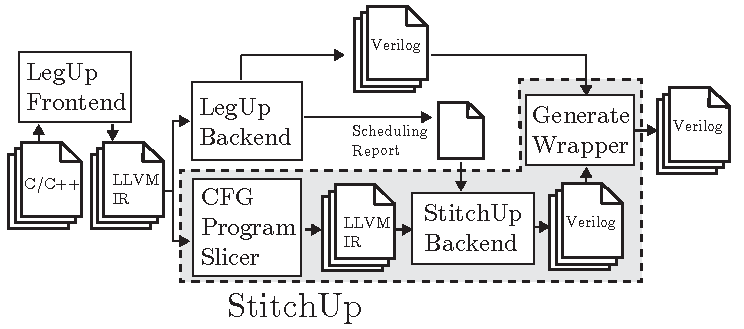
\includegraphics[width=3.5in]{./imgs/tool-flow.pdf}
\caption{Tool Flow Overview diagram}
\label{fig:tool_flow_diagram}
\end{figure}

%Flow Overview?
Figure \ref{fig:tool_flow_diagram} shows the transformation process from a C program
to a control-flow protected
Verilog hardware description, with StitchUp specific sections highlighted in grey.
Initially the C input is passed into the standard LegUp frontend, which is
a series of passes that
perform various tasks, such as annotating instructions with pipelining information.
This outputs an LLVM intermediate representation (LLVM-IR) which is passed both into the backend of LegUp,
to generate the
original unprotected circuit and also into the frontend of StitchUp to generate the control replicant circuit.
Finally an integration stage connects the original circuit to the duplicate control-flow circuit
and generates comparison logic to ensure that the state registers match.

%Why LegUp?
Our motivation for integrating our tool with LegUp is primarily due to it being open source, as
the StitchUp backend requires modification to the generation of the scheduling control FSMs.
However, the technique itself could be incorporated in VivadoHLS and all other HLS tools through modifying the
generated control FSM in a different fashion, (such as modifying the output HDL directly).
It is common for modern HLS tool to be constructed on top of LLVM-IR which has
a similar level of abstraction to assembly code.
It also has two important features for writing compiler optimisations:
first, all instructions are in single static assignment form (SSA) where every variable is only
assigned once; and second, instructions are grouped into straight-line sequences known as basic blocks (BB)
where there is only one entry branch at the very start of the block, and one exit branch at the very end.

\begin{figure}[t]
\centering
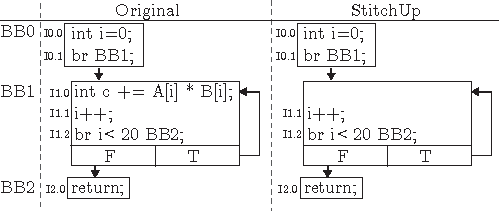
\includegraphics[width=3.5in]{./imgs/dot_product_cdfg.pdf}
\caption{Control-Data-Flow Diagram for Matrix Multiplication example}
\label{fig:mmm_cdfg}
\end{figure}

\subsection{Extracting the Control Instruction Set}
LLVM-IR, which is passed into the frontend of StitchUp, is naturally arranged into a CDFG
where each node is a basic block and edges are branch between them.
An example of the CDFG from the dot product in listing \ref{lst:DotProduct}
is shown on the left side of Figure \ref{fig:mmm_cdfg}.
The StitchUp frontend performs a backwards analysis walking the CDFG from bottom to top, collecting any control flow
related instructions that may influence whether an edge transition is taken.

All instructions deemed to be control related are collected into what we refer to as a Control Structure Instruction Set ($CSIS$),
which can be used to generate a control replicant.
Each basic block, $i$, in the input CDFG will have it's own associated $CSIS_{i}$ containing all instructions that may effect
control-flow after this point in the program.
The overall $CSIS$ for the input is $CSIS_s$ where $s$ is the initial basic block of the input program.

Algorithm \ref{alg:CSIS-extraction} is used to construct the $CSIS$ for all nodes in the CDFG.
It requires a fixed point iteration until the set of all $CSIS$, $C_{CSIS}$ has reached a stable state
which can be seen in line 1-2.
Each iteration walks backwards from the final basic block of the CDFG to the start basic block, as seen in
line 3, and for each encountered the corresponding $CSIS$ is updated using the following rules:

%\vspace{-4pt}
\begin{enumerate}
    \setlength{\itemsep}{3pt}
    \setlength{\parskip}{0pt}
    \setlength{\parsep}{0pt}
    \item $Sucessor(B)$ returns the set of all basic blocks in the CDFG that follow on from the basic block $B$.
	  For all successor  $j$ of basic block $i$ this rule adds every element of $CSIS_j$ to $CSIS_i$.
    \item This adds all branch instructions for the current basic block, $i$, to $CSIS_i$ using
	  $TerminatingInstruction(i)$ a function which returns the final instruction from the basic block $i$.
    \item Finally any instruction within the current basic block ($i$) that is used as an operand ($op_{c}$) by an element of $CSIS_i$ is added to $CSIS_i$
\end{enumerate}
\vspace{-4pt}

\begin{algorithm}[t]
\caption{CSIS Extraction Static Analysis Algorithm
\label{alg:CSIS-extraction}}
    \begin{algorithmic}[1]
        \INPUT a program, $P$, which is a set of Basic Blocks, \{$BB_0$, ..., $BB_N$\}
        \OUTPUT $P'$ a program containing only the instructions $I_c$ that are part of the control structure.
        \Statex
        \While{$C_{CSIS}$ != $P_{CSIS}$}
            \State $P_{CSIS} \gets \{CSIS_{BB0}, \dots,  CSIS_{BBN}$\}
            \For{\textbf{each} $B \in \{BB_{N},\dots,BB_{0}\}$}
                \\\hrulefill
                \For{\textbf{each} $S \in Successor(B)$}\Comment{Rule 1}
                    \For{\textbf{each} $I_{c} \in CSIS_{S}$}
                        \State $CSIS_B \cup \{I_{c}\}$
                    \EndFor
                \EndFor
                \\\hrulefill

                \State $T \in TerminatingInstruction(B)$\Comment{Rule 2}
                \State $CSIS_{B} \cup \{T\}$
                \For{\textbf{each} $op \in T$}
                    \State $CSIS_{B} \cup \{op\}$
                \EndFor
                \\\hrulefill

                \For{\textbf{each} $I \in B$}\Comment{Rule 3}
                    \For{\textbf{each} $I_c \in CSIS_{B}$}
                        \For{\textbf{each} $op_c \in I_c$}
                            \If{$I = op_{c}$}
                                \State $CSIS_{B} \cup \{I\}$
                            \EndIf
                        \EndFor
                    \EndFor
                \EndFor
            \EndFor
	\State $P' \gets CSIS_{BB0}$
        \EndWhile
    \end{algorithmic}
\end{algorithm}

To demonstrate this we will apply Algorithm \ref{alg:CSIS-extraction} to the
dot product example in \ref{lst:DotProduct} to extract the control-flow structure, 
labelled StitchUp in \ref{fig:mmm_cdfg}. 
For each update to a $CSIS$, the label for the instruction added from \ref{fig:mmm_cdfg} is given 
along with the rule from Algorithm \ref{alg:CSIS-extraction} used to add it. 

%-------------------------------------------------------
\vspace{1mm}
\noindent
\textbf{Initially} $CSIS_{i} = \emptyset$ for all basic blocks $i$

\vspace{-2mm}
\noindent
\hrulefill

\vspace{-1mm}
\noindent
\textbf{Iteration 1:}

%----BB2----
\FirstAnalysisTraceRule{BB2}{I2.0:\textbf{return}}{2}
\CSISState{BB2}{I2.0}
%----BB1----
\FirstAnalysisTraceRule{BB1}{every element in $CSIS_{BB2}$}{1}
\AnalysisTraceRule{I1.2:\textbf{br i<20 BB2}}{2}
\AnalysisTraceRule{I1.1:\textbf{i++}}{3}
\CSISState{BB1}{I2.0,I1.2,I1.1}
%----BB0----
\FirstAnalysisTraceRule{BB0}{every element in $CSIS_{BB1}$}{1}
\AnalysisTraceRule{I0.1:\textbf{br BB1}}{2}
\AnalysisTraceRule{I0.0:\textbf{i=0}}{3}
\CSISState{BB0}{I2.0,I1.2,I1.1,I0.1,I0.0}

\vspace{1mm}
\noindent
\textbf{Iteration 2:}\hspace{3mm} No Change, fixed point reached
%-----------------------------------------------------

\vspace{1mm}

Once the analysis is completed the final value of $CSIS_{BB0}$ is turned into LLVM-IR
and given to the StitchUp backend.
Here scheduling information from the original unmodified LegUp flow is used to generate
an identical control FSM to the original circuit and insert state lost scheduling states
due to instructions being removed. 
Finally, an integration stage takes the original LegUp and StitchUp circuits,
adds comparison logic to compare the state registers of the two circuits in each cycle,
and generates a top level wrapper to connect them
